%%%%%%%%%%%%%%%%%%%%%%%%%%%%%%%%%%%%%%%
% Wenneker Resume/CV
% LaTeX Template
% Version 1.1 (19/6/2016)
%
% This template has been downloaded from:
% http://www.LaTeXTemplates.com
%
% Original author:
% Frits Wenneker (http://www.howtotex.com) with extensive modifications by 
% Vel (vel@LaTeXTemplates.com)
%
% License:
% CC BY-NC-SA 3.0 (http://creativecommons.org/licenses/by-nc-sa/3.0/
%
%%%%%%%%%%%%%%%%%%%%%%%%%%%%%%%%%%%%%%

%----------------------------------------------------------------------------------------
%	PACKAGES AND OTHER DOCUMENT CONFIGURATIONS
%----------------------------------------------------------------------------------------

\documentclass[a4paper,10pt]{memoir} % Font and paper size

\usepackage{bibentry}
\makeatletter\let\saved@bibitem\@bibitem\makeatother
\usepackage{hyperref}
\makeatletter\let\@bibitem\saved@bibitem\makeatother



\newcommand\publication[1]{%
	\smallskip\par\hangpara{1.5em}{1}\bibentry{#1}\smallskip
}


%%%%%%%%%%%%%%%%%%%%%%%%%%%%%%%%%%%%%%%%%
% Wenneker Resume/CV
% Structure Specification File
% Version 1.1 (19/6/2016)
%
% This file has been downloaded from:
% http://www.LaTeXTemplates.com
%
% Original author:
% Frits Wenneker (http://www.howtotex.com) with extensive modifications by 
% Vel (vel@latextemplates.com)
%
% License:
% CC BY-NC-SA 3.0 (http://creativecommons.org/licenses/by-nc-sa/3.0/)
%
%%%%%%%%%%%%%%%%%%%%%%%%%%%%%%%%%%%%%%%%%

%----------------------------------------------------------------------------------------
%	PACKAGES AND OTHER DOCUMENT CONFIGURATIONS
%----------------------------------------------------------------------------------------

\usepackage{XCharter} % Use the Bitstream Charter font
\usepackage[utf8]{inputenc} % Required for inputting international characters
\usepackage[T1]{fontenc} % Output font encoding for international characters

\usepackage[top=1cm,left=1cm,right=1cm,bottom=1cm]{geometry} % Modify margins

\usepackage{graphicx} % Required for figures

\usepackage{flowfram} % Required for the multi-column layout

\usepackage{url} % URLs

\usepackage[usenames,dvipsnames]{xcolor} % Required for custom colours

\usepackage{tikz} % Required for the horizontal rule

\usepackage{enumitem} % Required for modifying lists
\setlist{noitemsep,nolistsep} % Remove spacing within and around lists

\setlength{\columnsep}{\baselineskip} % Set the spacing between columns

% Define the left frame (sidebar)
\newflowframe{0.2\textwidth}{\textheight}{0pt}{0pt}[left]
\newlength{\LeftMainSep}
\setlength{\LeftMainSep}{0.2\textwidth}
\addtolength{\LeftMainSep}{1\columnsep}
 
% Small static frame for the vertical line
\newstaticframe{1.5pt}{\textheight}{\LeftMainSep}{0pt}
 
% Content of the static frame with the vertical line
\begin{staticcontents}{1}
\hfill
\tikz{\draw[loosely dotted,color=RoyalBlue,line width=1.5pt,yshift=0](0,0) -- (0,\textheight);}
\hfill\mbox{}
\end{staticcontents}
 
% Define the right frame (main body)
\addtolength{\LeftMainSep}{1.5pt}
\addtolength{\LeftMainSep}{1\columnsep}
\newflowframe{0.7\textwidth}{\textheight}{\LeftMainSep}{0pt}[main01]

\pagestyle{empty} % Disable all page numbering

\setlength{\parindent}{0pt} % Stop paragraph indentation

%----------------------------------------------------------------------------------------
%	NEW COMMANDS
%----------------------------------------------------------------------------------------

\newcommand{\userinformation}[1]{\renewcommand{\userinformation}{#1}} % Define a new command for the CV user's information that goes into the left column

\newcommand{\cvheading}[1]{{\Huge\bfseries\color{RoyalBlue} #1} \par\vspace{.6\baselineskip}} % New command for the CV heading
\newcommand{\cvsubheading}[1]{{\Large\bfseries #1} \bigbreak} % New command for the CV subheading

\newcommand{\Sep}{\vspace{1em}} % New command for the spacing between headings
\newcommand{\SmallSep}{\vspace{0.5em}} % New command for the spacing within headings

\newcommand{\aboutme}[2]{ % New command for the about me section
\textbf{\color{RoyalBlue} #1}~~#2\par\Sep
}
	
\newcommand{\CVSection}[1]{ % New command for the headings within sections
{\Large\textbf{#1}}\par
\SmallSep % Used for spacing
}

\newcommand{\CVItem}[2]{ % New command for the item descriptions
\textbf{\color{RoyalBlue} #1}\par
#2
\SmallSep % Used for spacing
}

\newcommand{\bluebullet}{\textcolor{RoyalBlue}{$\circ$}~~} % New command for the blue bullets
 % Include the file specifying document layout and packages

%----------------------------------------------------------------------------------------
%	NAME AND CONTACT INFORMATION 
%----------------------------------------------------------------------------------------

\userinformation{ % Set the content that goes into the sidebar of each page
\begin{flushright}
% Comment out this figure block if you don't want a photo
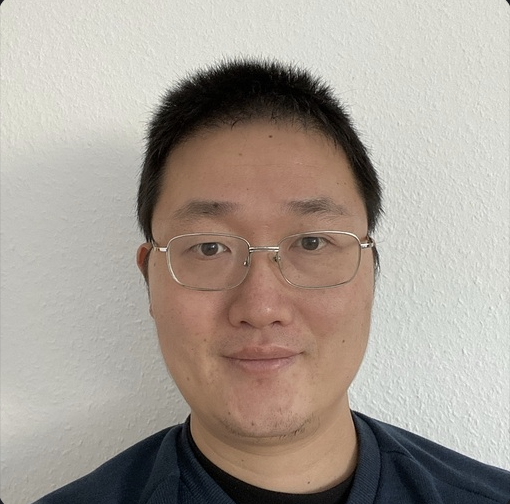
\includegraphics[width=0.9\columnwidth]{shuanglong}\\[\baselineskip] % Your photo
\small % Smaller font size
Shuanglong Kan \\ % Your name
\href{kanshuanglong@outlook.com}{kanshuanglong@outlook.com} \\ % Your email address
+49 1738938642
    
\Sep % Some whitespace
\textbf{Address} \\
Über den Bächelwiesen 15B\\ % Address 1
67691 Hochspeyer	 \\ % Address 2
Germany \\ % Address 3
\vfill % Whitespace under this block to push it up under the photo
\end{flushright}
}

%----------------------------------------------------------------------------------------

\begin{document}
	\nobibliography{cv.bib}
	\bibliographystyle{plain}
	

\userinformation % Print your information in the left column

\framebreak % End of the first column

%----------------------------------------------------------------------------------------
%	HEADING
%----------------------------------------------------------------------------------------

\cvheading{Shuanglong Kan} % Large heading - your name

\cvsubheading{Computer Scientist} % Subheading - your occupation/specialization

%----------------------------------------------------------------------------------------
%	Objective
%----------------------------------------------------------------------------------------

\aboutme{Background}{I am a computer scientist focusing on solving safety and security challenges in programming languages and compilers. Some of my representative works are as follows:
	\begin{itemize}
		\item A certified SMT solver for string data types. The solver algorithms are formalized and proved correct in Isabelle/HOL. Isabelle automatically generates the executable code in OCaml from verified algorithms.
		\item A certified compiler for SIGNAL language. SIGNAL is a synchronous language designed for embedded systems. The low-level code generation procedure is mathematically verified by \href{http://www.event-b.org/}{Event-B}. Event-B is a formal modeling and verification tool supporting refinement-based system development.
		\item A front-end for C language to automatically support code instruments for testing. For some special testing requirements, the tool automatically inserts testing code.
		\item The verification-oriented compilers for Rust and Solidity languages. The compilers translate Rust or Solidity programs to mathematical formulas, and we then leverage mathematical tools to reason the  programs' correctness automatically.
	\end{itemize}
	
	Most of my works are published in top-tier conferences, such as POPL (ACM SIGPLAN Symposium on Principles of Programming Languages), ISSTA (ACM SIGSOFT International Symposium on Software Testing and Analysis), S\&P (IEEE Symposium on Security and Privacy). 
}

%----------------------------------------------------------------------------------------
%	EDUCATION
%----------------------------------------------------------------------------------------

\CVSection{Education}

%------------------------------------------------

\CVItem{Sep. 2011 - Jun. 2017, Nanjing University of Aeronautics and Astronautics, China
}{Doctor of Computer Science. Supervisor: Prof. Zhiqiu Huang} 

Thesis: Research on the Trustworthy Code Generation from SIGNAL

\begin{itemize}
	\item \href{http://polychrony.inria.fr/}{SIGNAL} is a mathematical modeling language for distributed reactive system.
	\item Design a multi-threaded code generation from SIGNAL.
	\item Mathematically prove  the correctness of the code generation in \href{http://www.event-b.org/}{Event-B}.
	\item Develop model checking techniques for state machines.
\end{itemize}
~\\
%------------------------------------------------
\CVItem{Jan.2016 - Jun. 2016, IRIT, University Toulouse III, France
}{Visiting Researcher. Supervisor: Prof. Jean-Paul Bodeveix and Mamoun Filali}

Project: Certified code generation from SIGNAL.
~\\



\CVItem{Sep. 2007 - Jun. 2011, Nanjing University of Aeronautics and Astronautics, China}{Bachelor of Computer Science}
%------------------------------------------------

\Sep % Extra whitespace after the end of a major section

%----------------------------------------------------------------------------------------
%EXPERIENCE
%----------------------------------------------------------------------------------------

\CVSection{Work Experience}

%------------------------------------------------

\CVItem{01.11.2022 - now, Senior  Software Engineer in \href{https://www.certik.com/}{Certik}, remote work, a Web3 Security company focusing smart contracts and cryptography.}{
Certik is a leading web3 security company located in New York, US.\\
Project:  A verification-oriented compiler for Solidity language
\begin{itemize}
	\item Design the architecture of smart contract formal verification tools. 
	\item Design reusable Intermediate Representation (IR) for smart contracts formal verification.
	\item Develop model checking techniques for smart contracts.
	\item Develop deductive verification techniques for smart contracts.
\end{itemize}
Smart contracts are snippets of code integrated into blockchains to support financial activities. 
Vulnerabilities in smart contracts may yield billions of dollars being hacked.
}


\CVItem{15.10. 2019 - 31.10.2022, \textit{Research Assistant}, TU Kaiserslautern, Germany}
{
Project: A Certified mathematical reasoning tool for string types in programming languages. Supervisor Anthony W. Lin
\begin{itemize}
	
	\item I developed a certified string solver using Isabelle interactive theorem prover, which can be widely used in programming language verification. Amazon AWS and Microsoft Azure also use string solvers heavily for access control policies.

\item Certified Software means the software is mathematically proved by interactive theorem prover, such as \href{https://coq.inria.fr/}{Coq} and \href{https://isabelle.in.tum.de/}{Isabelle}. 
	
\item \href{https://compcert.org/}{Compcert} C compiler and \href{https://sel4.systems/}{sel4} operating system are developed by Coq and Isabelle respectively to provide high-assured compiler and operating systems.



\end{itemize}

More info:
SMT solvers, such as \href{https://github.com/Z3Prover/z3}{z3}, and \href{https://cvc5.github.io/}{CVC5} are widely used in providing automated reasoning power for computer systems. Tools, such as \href{https://frama-c.com/}{Frama-C},  Event-B,  Software Model checkers (such as \href{https://monteverdi.informatik.uni-freiburg.de/tomcat/Website/}{Ultimate}, 
\href{https://cpachecker.sosy-lab.org/}{CPAChecker}, and \href{https://www.cprover.org/cbmc/}{CBMC}) are all based on SMT solvers.
}

\clearpage % Start a new page

\userinformation % Print your information in the left column

\framebreak % End of the first column

\CVItem{01.09.2017 - 30.09.2019, \textit{Research Fellow}, Nanyang Technological University, Singapore}{
	Project: A verification-oriented compiler for Rust language.
	Supervisor Yang Liu and Shang-wei Lin
	\begin{itemize}
		\item Rust is a programming language aiming for replacing C and non-memory errors. 
		\item I developed the security vulnerability detection tools for Rust  using \href{https://kframework.org/}{K-Framework}, which is a rewriting-logic based semantics modeling tool.
	\end{itemize}
}

%------------------------------------------------




%----------------------------------------------------------------------------------------
%	NEW PAGE DELIMITER
%	Place this block wherever you would like the content of your CV to go onto the next page
%----------------------------------------------------------------------------------------



\CVSection{Teaching}


\CVItem{The Principles of Compiler Design}{Summer semester 2012, Nanjing University of Aeronautics and Astronautics, China}

\CVItem{Software Metrics}{Winter semester 2013, Nanjing University of Aeronautics and Astronautics, China}

\CVItem{Software Testing}{Summer semester 2018, Nanyang Technological University, Singapore}

\CVItem{An Introduction to Isabelle Interactive  Proof Assistant}{Department of Computer Science, Summer semester 2021, TU Kaiserslautern, Germany}

\CVItem{Logic and Verification Seminar}{Department of Computer Science, Summer semester 2021, TU Kaiserslautern, Germany}


\CVItem{An Introduction to Isabelle Interactive  Proof Assistant}{Department of Computer Science, Summer semester 2020, TU Kaiserslautern, Germany}

\CVItem{Logic and Verification Seminar}{Department of Computer Science, Summer semester 2020, TU Kaiserslautern, Germany}





%----------------------------------------------------------------------------------------

\Sep % Extra whitespace after the end of a major section

\CVSection{Fellowships/Awards}

%------------------------------------------------

\CVItem{2016, \textit{Visiting PhD student Scholarship}, Nanjing University of Aeronautics and Astronautics}{The scholarship covers all my expense for the academic visiting in Toulouse, France}


\CVItem{2017, \textit{Excellent Doctor degree dissertation}, Nanjing University of Aeronautics and Astronautics}{For my PhD thesis: Research on the Trustworthy Code Generation from SIGNAL}


\CVItem{2019, \textit{ISSTA Distinguished Paper Award}}{The ACM SIGSOFT International Symposium on Software Testing and Analysis (ISSTA) is the leading research symposium on software testing and analysis}


\CVItem{2022, \textit{CPP Distinguished Paper Award}}{Certified Programs and Proofs (CPP) is an international conference on practical and theoretical topics in all areas that consider formal verification and certification as an essential paradigm for their work}

\CVItem{2023, \textit{SMT-COMP 2023 (Satisfiability Modulo Theories Competition) Winner of the Logic String}}{SMT-COMP is the most important contest in SMT community.}
%------------------------------------------------

\Sep % Extra whitespace after the end of a major section


\CVSection{Skills}{

%------------------------------------------------
I am an expert of the following languages and tools.
\begin{itemize} 
	\item Programming languages: C, C\#, Python, Java, Rust, Solidity (smart contract language), OCaml.
	\item Github, Docker and AWS
	\item Event-B, which is a formal method for system-level modelling and analysis.
    \item \href{https://www.cs.bu.edu/~hwxi/atslangweb/}{ATS} is a functional-like programming language that generates corresponding C code for low-level applications. You can mathematically prove an ATS program bug-free, and this proof will guarantee the generated C code is also bug-free. 
    \item Isabelle interactive theorem prover, with which I developed a certified sequence solver.
    \item Coq proof assistant. Coq also supports dependent type as ATS.
	\end{itemize}
	}
%----------------------------------------------------------------------------------------
%----------------------------------------------------------------------------------------


\clearpage % Start a new page

\userinformation % Print your information in the left column

\framebreak % End of the first column

\Sep % Extra whitespace after the end of a major section

\CVSection{Publications}

%------------------------------------------------

\textbf{Conference Papers}
\begin{enumerate}
	\item \publication{chen2022solving} 
	 \item \publication{KanLRS22}
	 \item \publication{DBLP:conf/sp/JiaoK0S0020}
	\item \publication{DBLP:conf/issta/ChenYKQX19}
	\item \publication{DBLP:conf/sigsoft/Kan14}
	\item \publication{DBLP:conf/icfem/KanHC16}
	\item \publication{DBLP:conf/memocode/BodeveixFK17}
	\item \publication{DBLP:conf/iceccs/JiangSZK019}
\end{enumerate}
~\\\\

\textbf{Journal Papers}

\begin{enumerate}
	\item \publication{yin2021safeosl}
	\item \publication{DBLP:journals/logcom/KanHCLH17}
	\item \publication{DBLP:journals/cj/KanH18}
	\item \publication{DBLP:journals/spe/KanH18}
	\item \publication{DBLP:journals/compsec/HuZLZKC21}
	\item \publication{DBLP:journals/access/LiKH17}
\end{enumerate}
\clearpage % Start a new page

\userinformation % Print your information in the left column

\framebreak % End of the first column

\Sep % Extra whitespace after the end of a major section

\begin{enumerate}
	\setcounter{enumi}{6}
	\item \publication{yan2018location}
	\item \publication{kan2014bounded}(in Chinese)
\end{enumerate}

%------------------------------------------------



%----------------------------------------------------------------------------------------

\CVSection{Projects}
\begin{enumerate}
	\item Research on Verification for the Memory Safety Mechanisms of Rust, Young Scientists Fund of the National Natural Science Foundation of China (PI) 250,000 CNY
	\item Securify: A compositional Approach of Building Security Verified System, \url{http://securify.sce.ntu.edu.sg/}(Participant)
	\item Research on Privacy Modeling and Verification in Evolving Cloud Computing, National Natural Science Foundation of China (Participant)
\end{enumerate}

\Sep

\CVSection{Student Supervision}

\begin{enumerate}
	\item Xiaohua Yin (PhD student in Nanjing University of Aeronautics and Astronautics, China)
	\item Xinwen Hu (PhD student in Nanjing University of Aeronautics and Astronautics, China)
	\item Micha Schrader (Master student in TU Kaiserslautern, Germany)
\end{enumerate}

\Sep

\CVSection{Services}{ }

Assisting my supervisor in reviewing submissions from TACAS 2018, CCS 2018, FTSCS 2018, ATVA 2018.
Subreviewer of CSL 2022.

\Sep

\CVSection{Languages (Common European Framework of
	Reference for languages (CEFR))}{
%------------------------------------------------
\begin{itemize} 

    \item English C1.2 Level
    \item German A2 Level, and now learning B1.
    
  \end{itemize}
    	}
\Sep % Extra whitespace after the end of a major section
\end{document}
